\documentclass[]{article}
\usepackage{lmodern}
\usepackage{amssymb,amsmath}
\usepackage{ifxetex,ifluatex}
\usepackage{fixltx2e} % provides \textsubscript
\ifnum 0\ifxetex 1\fi\ifluatex 1\fi=0 % if pdftex
  \usepackage[T1]{fontenc}
  \usepackage[utf8]{inputenc}
\else % if luatex or xelatex
  \ifxetex
    \usepackage{mathspec}
  \else
    \usepackage{fontspec}
  \fi
  \defaultfontfeatures{Ligatures=TeX,Scale=MatchLowercase}
\fi
% use upquote if available, for straight quotes in verbatim environments
\IfFileExists{upquote.sty}{\usepackage{upquote}}{}
% use microtype if available
\IfFileExists{microtype.sty}{%
\usepackage{microtype}
\UseMicrotypeSet[protrusion]{basicmath} % disable protrusion for tt fonts
}{}
\usepackage{hyperref}
\PassOptionsToPackage{usenames,dvipsnames}{color} % color is loaded by hyperref
\hypersetup{unicode=true,
            pdftitle={Self-Replicating Functions},
            pdfauthor={Tyler Neylon},
            colorlinks=true,
            linkcolor=black,
            citecolor=Blue,
            urlcolor=Blue,
            breaklinks=true}
\urlstyle{same}  % don't use monospace font for urls
\usepackage{graphicx,grffile}
\makeatletter
\def\maxwidth{\ifdim\Gin@nat@width>\linewidth\linewidth\else\Gin@nat@width\fi}
\def\maxheight{\ifdim\Gin@nat@height>\textheight\textheight\else\Gin@nat@height\fi}
\makeatother
% Scale images if necessary, so that they will not overflow the page
% margins by default, and it is still possible to overwrite the defaults
% using explicit options in \includegraphics[width, height, ...]{}
\setkeys{Gin}{width=\maxwidth,height=\maxheight,keepaspectratio}
\IfFileExists{parskip.sty}{%
\usepackage{parskip}
}{% else
\setlength{\parindent}{0pt}
\setlength{\parskip}{6pt plus 2pt minus 1pt}
}
\setlength{\emergencystretch}{3em}  % prevent overfull lines
\providecommand{\tightlist}{%
  \setlength{\itemsep}{0pt}\setlength{\parskip}{0pt}}
\setcounter{secnumdepth}{5}
% Redefines (sub)paragraphs to behave more like sections
\ifx\paragraph\undefined\else
\let\oldparagraph\paragraph
\renewcommand{\paragraph}[1]{\oldparagraph{#1}\mbox{}}
\fi
\ifx\subparagraph\undefined\else
\let\oldsubparagraph\subparagraph
\renewcommand{\subparagraph}[1]{\oldsubparagraph{#1}\mbox{}}
\fi
\usepackage{subfig}
\AtBeginDocument{%
\renewcommand*\figurename{Figure}
\renewcommand*\tablename{Table}
}
\AtBeginDocument{%
\renewcommand*\listfigurename{List of Figures}
\renewcommand*\listtablename{List of Tables}
}
\usepackage{float}
\floatstyle{ruled}
\makeatletter
\@ifundefined{c@chapter}{\newfloat{codelisting}{h}{lop}}{\newfloat{codelisting}{h}{lop}[chapter]}
\makeatother
\floatname{codelisting}{Listing}
\newcommand*\listoflistings{\listof{codelisting}{List of Listings}}

\title{Self-Replicating Functions}
\author{Tyler Neylon}
\date{204.2016}

\begin{document}
\maketitle

These are notes I'm creating for myself as I explore functions \(f\)
that can be written as a sum \(f = g_1 + g_2\) where \(g_1\) and \(g_2\)
are the same up to symmetry, and both \(g_1\) and \(g_2\) strongly
resemble shifts of the original function \(f\). When a function \(f\)
has these properties, I informally call it a \emph{self-replicating
function}.

Like the word \emph{fractal}, this term is not rigorously defined --- in
particular, it depends on the ambiguous notion of ``strong resemblance''
--- although I plan to investigate more precise requirements below.

\begin{figure}[htbp]
\centering
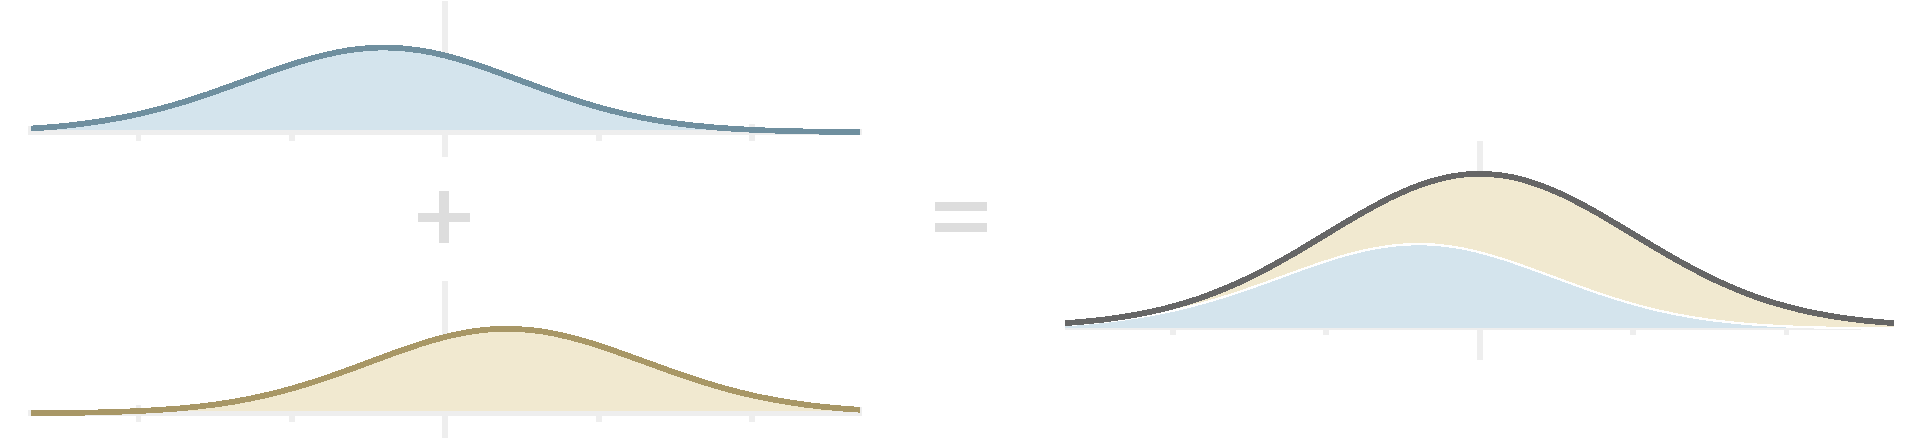
\includegraphics{images/pdfs/added_normals4.pdf}
\caption{\label{fig:added_normals}As an example of a self-replicating
function, the normal curve can be expressed as the sum of two
normal-like curves that are reflections of each
other.}\label{fig:addedux5fnormals}
\end{figure}

\section{Motivation}\label{motivation}

I became interested in self-replicating functions by working on
algorithms to procedurally generate 3d models of natural-looking trees.
When algorithmically making trees, it makes sense to start from the idea
of an \href{https://en.wikipedia.org/wiki/L-system}{\emph{L-system}},
which can be visualized as a kind of fractal in which a trunk forks into
branches that themselves fork into smaller subranches, this process
repeating infinitely.

I noticed that tree-like \emph{L}-systems can have a large amount of
``branch overlap'' concentrated around a central area of their apparent
surface. For example, consider the two images in
figure~\ref{fig:ellsystem}. On the left is a standard \emph{L}-system
along with a histogram showing the density of leaf points along the
edge. Intuitively, the leaf points are dense even toward the extreme
angles of the tree's top. However, the density increases continuously
toward the center.

We could think of each leaf point as doing a certain amount of work by
covering some area along the top of the \emph{L}-system. Each subtree is
so oblivious to its other subtrees that they overlap heavily, and the
central leaf points end up being highly redundant. To illustrate this
redundancy, the right-hand figure shows the exact same \emph{L}-system
with essentially half of the tree removed --- yet the shape formed by
the leaf points is only slightly changed.

\begin{figure}[htbp]
\centering
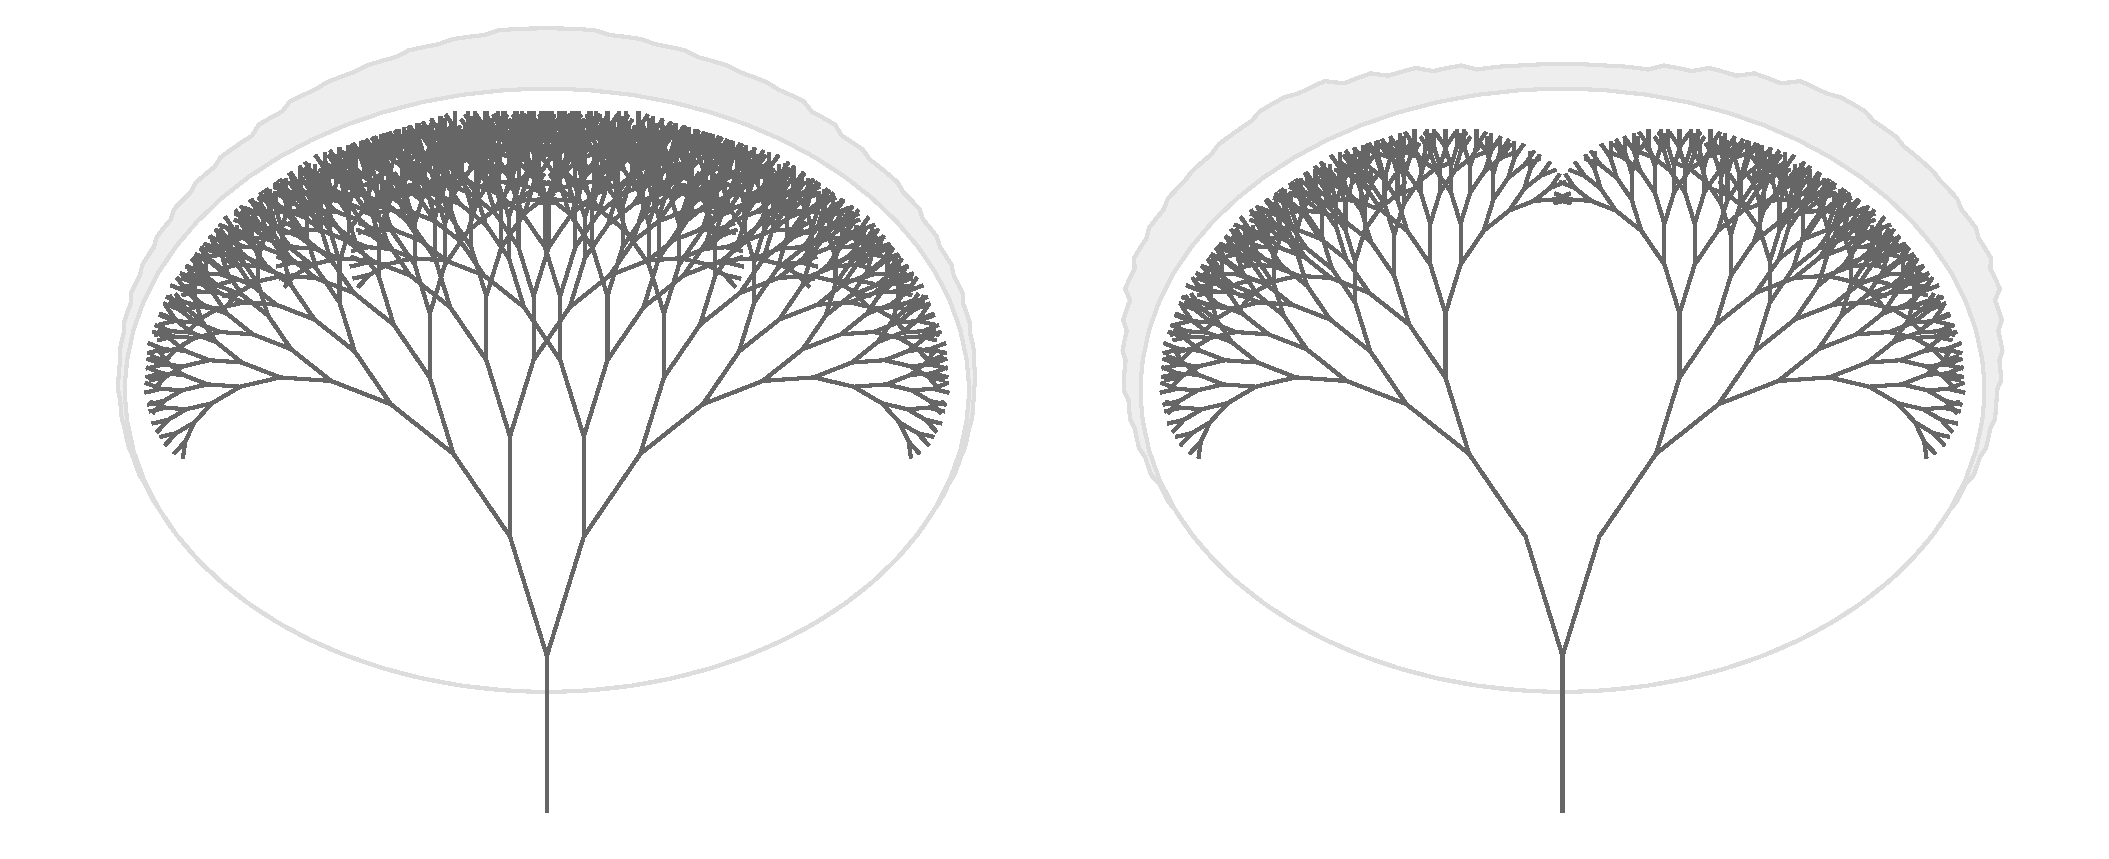
\includegraphics{images/pdfs/ellsystem2.pdf}
\caption{\label{fig:ellsystem}Left: An \emph{L}-system; Right: the same
system with two large subtrees removed. In both cases, a histogram of
leaf point density is provided around an outer
ellipse.}\label{fig:ellsystem}
\end{figure}

One approach to smoothing out the distribution of leaf points would be
to compromise the fractal-like nature of the system by choosing each
line direction based on where it is within the fractal, rather than
simply by making each branching point a smaller version of its parent.
The line directions can be chosen so that the set of points at a fixed
distance from the trunk point form a set of equidistant angles from a
central point. The result is an extremely regular edge, as seen in
figure~\ref{fig:well_dist}.

\begin{figure}[htbp]
\centering
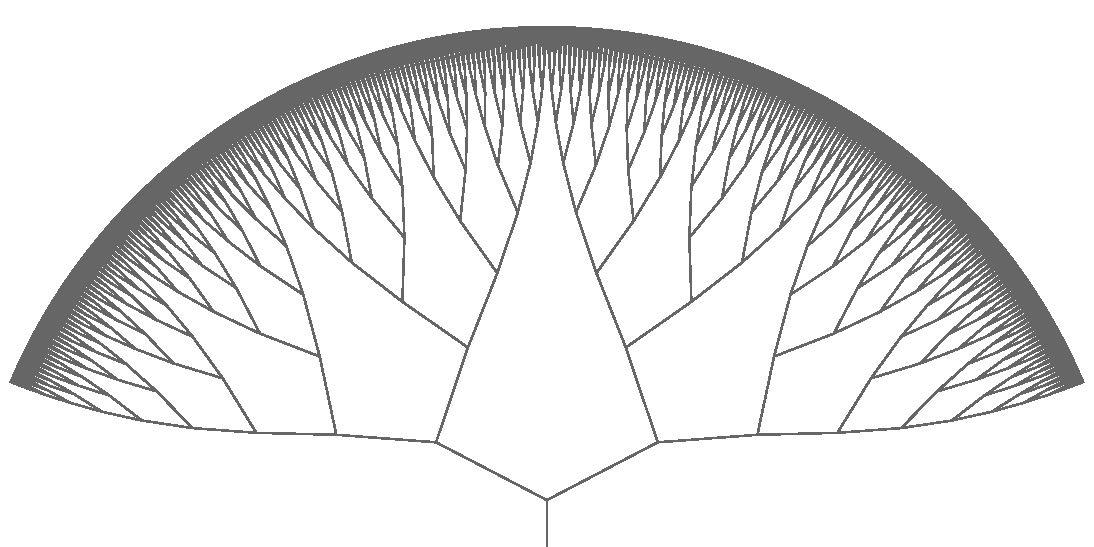
\includegraphics{images/pdfs/well_distributed_ell_like_system.pdf}
\caption{\label{fig:well_dist}A \emph{L}-like system in which line
directions are chosen to maximize the regularity of leaf point
distribution.}\label{fig:wellux5fdist}
\end{figure}

This is ideally efficient in that each leaf point is equally important
in forming the shape of the system. However, this system is defined in
terms of the path to each point. Is it possible to design a system so
that the overall distribution of leaf points is fairly even, yet each
subtree's shape is independent of its position within the full tree?

If this goal were achieved, we would necessarily have a leaf point
distribution which was the sum of two smaller versions of itself.
Intuitively, the leaf-point distribution of any \emph{L}-system is
already a self-replication function because, if its two main subtrees
have distribution functions \(g_1\) and \(g_2\), then the full tree has
distribution function \(f = g_1 + g_2\). I have to say
\emph{intuitively} here because I haven't formally defined the
leaf-point distribution of an \emph{L}-system.

Thus, \emph{L}-systems naturally coincide with self-replicating
functions. Although there are probably self-replicating functions which
do not correspond with \emph{L}-systems, I nonetheless find it
interesting to independently explore the world of self-replicating
functions.

\section{Simple cases}\label{simple-cases}

Technically, any polynomial can be seen as a kind of self-replicating
function. For example, if \(f(x) = x^2\),

\[\begin{array}{rcl}
  g_1(x) & = & (x + 1)^2 - 1 = x^2 + 2x, \quad \text{and} \\
  g_2(x) & = & (x - 1)^2 - 1 = x^2 - 2x, \\
\end{array}\]

then \(f = g_1 + g_2\), and each \(g_i\) is a shift of the original
function \(f\). In general, if \(f(x) = ax^n + O(x^{n-1})\) then we can
choose \(g_i(x) = a(x\pm 1)^n + O(x^{n-1})\) so that \(f = g_1 + g_2\),
and each \(g_i\) has

\[ \lim_{x\to\pm\infty}\frac{g_i(x)}{f(x)} = 1,\]

which is good enough for me to subjectively say that they strongly
resemble shifts of \(f\).

However, the original motivation for self-replicating functions is based
on distribution functions, so the rest of this note focuses on functions
\(f\) for which \(\lim_{x\to\pm\infty}f(x) = 0\).

Another simple approach would be to set \(g_1 = g_2 = \frac{1}{2}f\) for
any function \(f\). This is not very interesting, and the word
\emph{shift} in the informal definition of a self-replicating function
is intended to defeat this trivial case. That is, each \(g_i\) is
expected to be similar to a translation of \(f\), such as \(f(x-1)\) or
\(f(x+1)\).

\subsection{Indicator functions}\label{indicator-functions}

The next function I'll describe is simple and meets all of the
requirements so far. An \emph{indicator function} is a function taking
on only the value 0 or 1; it's also sometimes referred to as a
\emph{characteristic function}. If \(f\) is an indicator function, then
you can think of those \(x\) with \(f(x) = 1\) as belonging to the
subset of the domain which is \emph{indicated} by the function. It's
handy to use the following bracket notation of Knuth and others: given
any boolean predicate \(P(x)\), let \([P(x)]\) denote the value 1 when
\(P(x)\) is true, and false otherwise (Knuth 1998).

Given a half-open interval \([a, b)\), define \(I_{[a, b)}\) to be the
function \([x\in[a, b)]\). The following equation shows how such
indicator functions can be considered simple self-replicating functions:
\(I_{[0, 2)} = I_{[0, 1)} + I_{[1, 2)}\).

\begin{figure}[htbp]
\centering
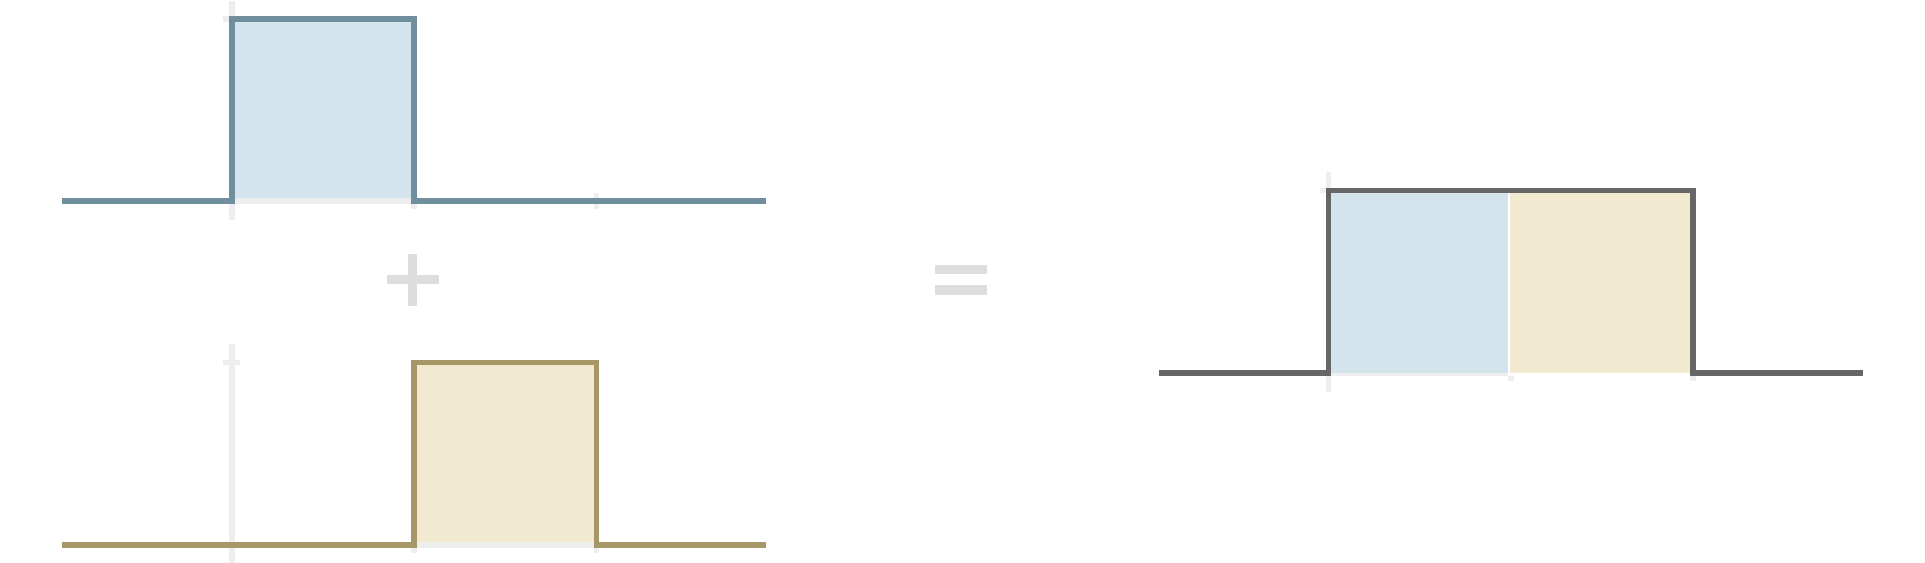
\includegraphics{images/pdfs/added_intervals6.pdf}
\caption{\label{fig:added_intervals}Visual representation of the
addition of indicator functions of
intervals.}\label{fig:addedux5fintervals}
\end{figure}

In order to match the equation \(f = g_1 + g_2\), emphasizing the
similarity between the \(g_i\)'s and \(f\), we can set
\(f = I_{[0, 2)}\), \(g_1 = f(2x) = I_{[0, 1)}\), and
\(g_2 = f(2(x - 1)) = I_{[1, 2)}\).

\subsection{Ramp functions}\label{sec:rampux5ffunctions}

Things get more interesting when \(g_1(x) g_2(x) \ne 0\) for some \(x\).
To this end, define the \emph{ramp function} for values \(a,b,c,d\) with
\(a < b < c < d\) via

\[ J_{a,b,c,d} = \begin{cases}
(x - a) / (b - a) & \text{if } x \in [a, b), \\
1 & \text{if } x \in [b, c), \\
(d - x) / (d - c) & \text{if } x \in [c, d), \text{and} \\
0 & \text{otherwise.} \\
\end{cases}\]

Then \(J_{0,1,4,5} = J_{0,1,2,3} + J_{2,3,4,5}\), as illustrated in
figure~\ref{fig:ramp_fns}.

\begin{figure}[htbp]
\centering
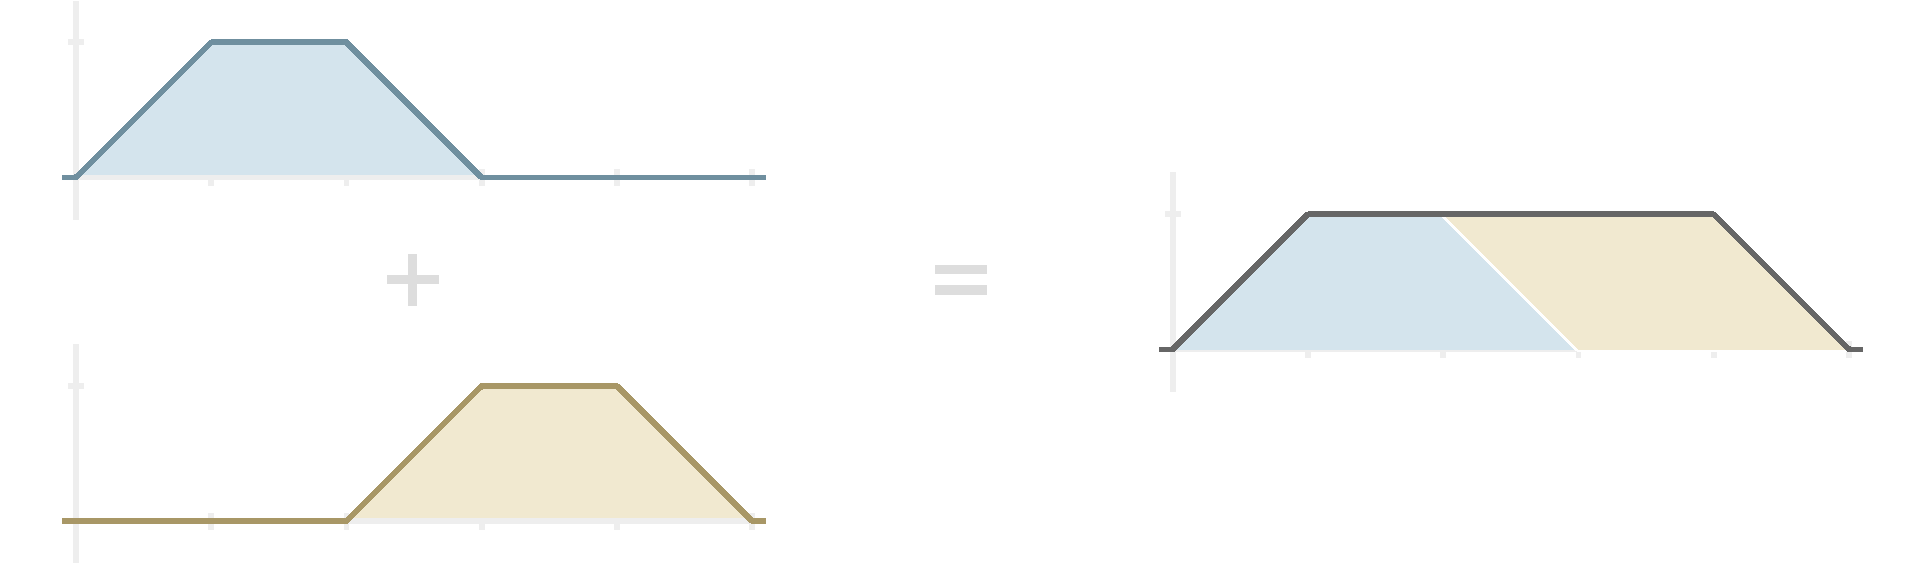
\includegraphics{images/pdfs/ramp_fns3.pdf}
\caption{\label{fig:ramp_fns}Visual addition of two ramp functions to
form another.}\label{fig:rampux5ffns}
\end{figure}

The ramp function example gives me four ideas for further study:

\begin{enumerate}
\def\labelenumi{\arabic{enumi}.}
\tightlist
\item
  The addends and the sum cannot be expressed as linearly related; that
  is, there is no linear function \(\ell(x)\) so that
  \(J_{0, 1, 2, 3}(\ell(x)) = J_{0, 1, 4, 5}(x)\). Contrast this with
  the interval functions where \(I_{[0, 1)}(x / 2) = I_{[0, 2)}\). This
  raises the questions: Which self-replicating functions allow for this
  linear-relation restriction? Is there a slight modification of ramp
  functions which meets this linear-relation restriction?
\item
  The ramp functions are piece-wise linear, but that linearity is not
  really the key to their being self-replicating. Rather, the key is
  that the left ramp and right ramp sum to 1, which matches the middle
  height of the functions. Which more general self-replicating functions
  can be constructed using this idea?
\item
  What happens if we treat the sum \(f = g_1 + g_2\) as part of a
  sequence? Thinking of \emph{L} and \emph{R} for \emph{left} and
  \emph{right}, let \(f^{(0)}_L = J_{0, 1, 2, 3}\), and
  \(f^{(i)}_R = f^{(i)}_L(x-2)\) for \(i \ge 0\). Thinking of \emph{S}
  for \emph{sum}, define \(f^{(i+1)}_S = f^{(i)}_L + f^{(i)}_R\) for
  \(i \ge 1\). If \(f^{(i)}_L\) is positive on \((0, b)\), then
  \(f^{(i)}_R\) is positive on \((2, b + 2)\), so \(f^{(i+1)}_S\) is
  positive on \((0, b + 2)\). Set
  \(f^{(i+1)}_L = f^{(i+1)}_S(x (b + 2) / b)\) so that we maintain the
  region on which the left function is positive. In this way, we get a
  sequence of functions. What is the limiting behavior? Can we attempt
  to extend the sequence backwards? Can we say anything in general about
  the limiting behavior of a class of starting functions \(f^{(0)}_L\)?
\item
  For the current ramp functions, the middle section is flat with value
  1, while the edges sum to 1. Can we do something more interesting
  where the edges sum to a non-constant value? I can imagine this
  leading to a discontinuous function. Is there a way to do this where
  the functions are continuous, or at least continuous almost
  everywhere? Can we describe a general class of self-replicating
  functions which are not continuous, such as the indicator function of
  the Cantor dust?
\end{enumerate}

TODO Mention how I'm following up with further study idea 1.

\subsection{Nonlinear ramps}\label{sec:nonlinearux5framps}

Other curves that sum to 1 could easily take the place of the left and
right edges of the ramp function. For example, the left and right ramps
could be replaced by curves with the shapes of \(x^2\) and \(1-x^2\) on
\(x\in [0, 1]\), as illustrated in figure~\ref{fig:nonlinear_ramps}.

\begin{figure}[htbp]
\centering
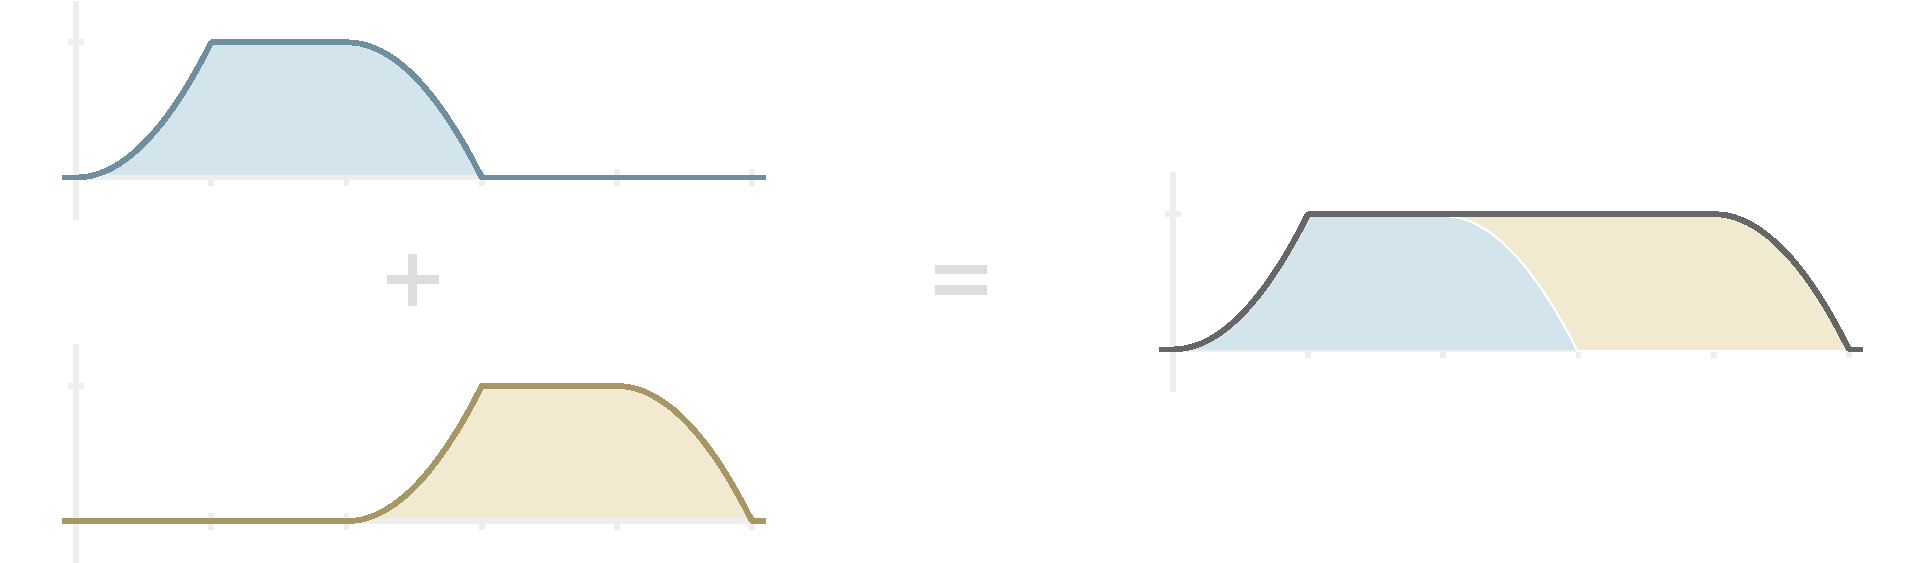
\includegraphics{images/pdfs/nonlinear_ramps2.pdf}
\caption{\label{fig:nonlinear_ramps}An example of nonlinear ramp
functions using \(x^2\) on \(x\in [0, 1]\) to determine the edge
shapes.}\label{fig:nonlinearux5framps}
\end{figure}

Given any function \(f:[0,1]\to [0,1]\), the generalized ramp function
is

\[ K_{a,b,c,d} = \begin{cases}
f\big((x - a) / (b - a)\big) & \text{if } x \in [a, b), \\
1 & \text{if } x \in [b, c), \\
1 - f\big((x - c) / (d - c)\big) & \text{if } x \in [c, d), \text{and} \\
0 & \text{otherwise.} \\
\end{cases}\]

If any function can be written as \(K_{a,b,c,d}\) for some value of
\(f\), I'll call it a \(K-\)\emph{function}. This form is general enough
to include interval functions --- for example, by using \(f(x) = 0\)
---~and to include the previous ramp function \(J(x)\) by setting
\(f(x)=x\).

The versatility of the \(K-\)functions shows that we can produce
self-replicating functions that are highly discontinuous, such as by
setting \(f(x)\) to be the indicator function of a set with many border
elements. Even among continuous functions, we can produce
self-replicating functions which avoid being ``mostly monotonic.'' In
particular, I'll say that a function \(f:\mathbb{R}\to\mathbb{R}\) is
\emph{peak monotonic} iff there is a point \(x\) such that
\(a < b < x \Rightarrow f(a) \le f(b)\) and
\(x < c < d \Rightarrow f(c) \ge f(d)\). The indicator function of an
interval and the ramp function are both peak monotonic, while the
example \(K-\)functions in figure~\ref{fig:other_ramps} are not.

\begin{figure}[htbp]
\centering
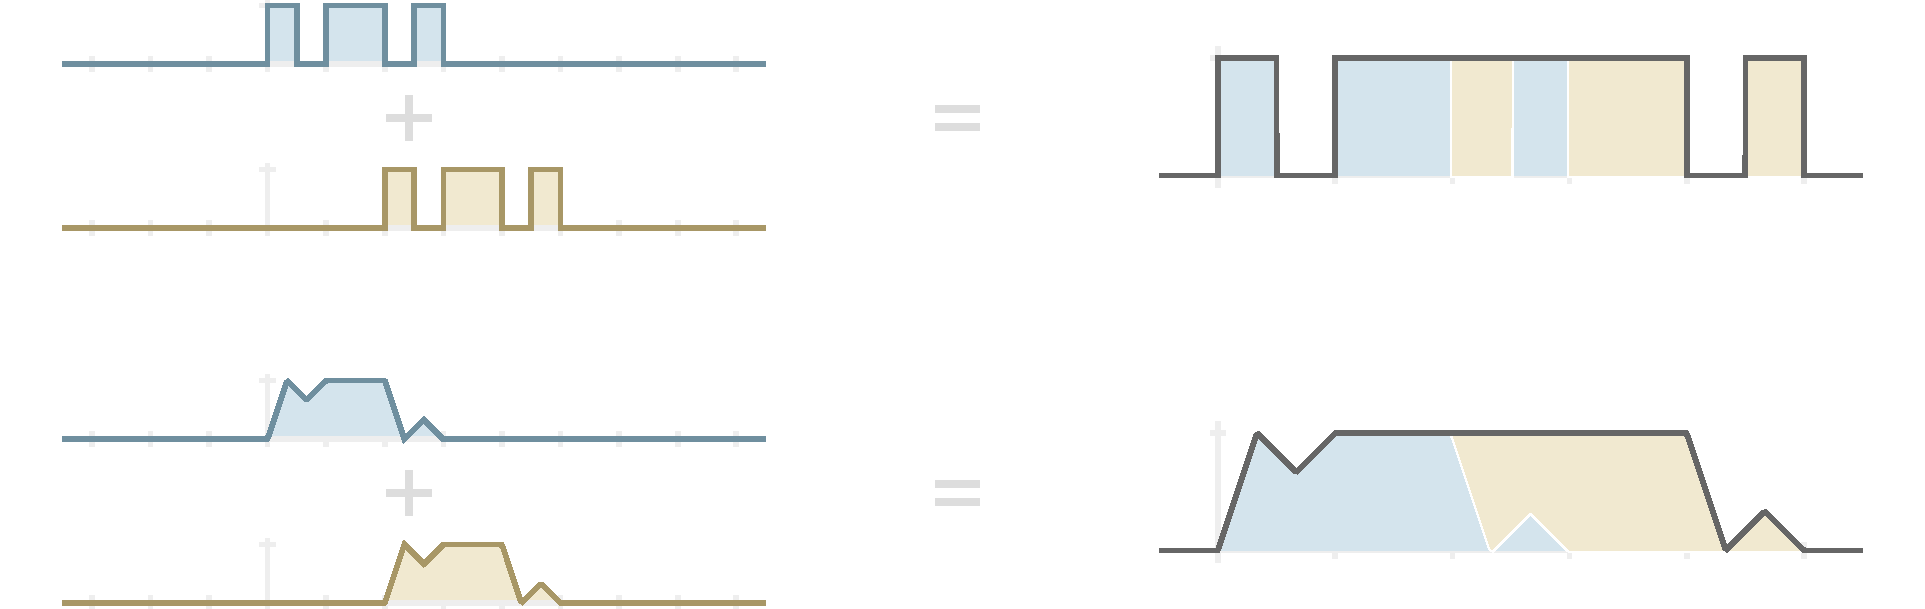
\includegraphics{images/pdfs/other_ramps2.pdf}
\caption{\label{fig:other_ramps}Example \(K-\)functions: on the top is a
function more discontinuous than the indicator function of an interval;
on the bottom is a continuous but non-peak-monotonic
function.}\label{fig:otherux5framps}
\end{figure}

\subsection{Non-plateau functions}\label{non-plateau-functions}

The ramp functions \(K_{a,b,c,d}\) all have the constant value 1 on the
middle interval \([b, c]\). This requires the ramps on intervals
\([a, b]\) and \([c, d]\) sum to 1. In this section, I'll consider what
can happen if we relax this condition. I'll informally call these
\emph{non-plateau functions}.

It will be useful to propose one possible formalization of a
self-replicating function before exploring non-plateau functions.

\subsubsection{A formal definition for self-replicating
functions}\label{a-formal-definition-for-self-replicating-functions}

I think the term \emph{self-replicating function} is best left as an
intuitive, non-rigorous concept because there seem to be a wide variety
of instances that are best studied via their own particular flavors of a
formal definition. A number of other terms used to discuss mathematics
are similarly unformalized or context-specific: consider \emph{fractal},
\emph{symmetry}, or \emph{closure} as examples. Nonetheless, many
self-replicating functions meet the conditions of the definition I'll
present next.

Call a function \(f\) \emph{exactly self-replicating} iff there exist
continuous bijections \(s\), \(t_1\), and \(t_2\) such that \(s\) is not
the identity function and

\begin{equation}\begin{array}{rcl}
  f_L(x) & = & f(x), \\
  f_R(x) & = & f(s(x)), \\
  f_S(x) & = & f_L(x) + f_R(x), \text{and} \\
  f_L(x) & = & t_2(f_S(t_1(x))).
\end{array}\label{eq:exact_defn}\end{equation}

The \emph{L}, \emph{R}, and \emph{S} subscripts are meant to hint that
these functions act as the \emph{left} addend, \emph{right} addend, and
the \emph{sum}; the \(s\) function suggests a \emph{shift}, while the
\(t_1\) and \(t_2\) functions suggest a \emph{transformation}. The last
equation in (\ref{eq:exact_defn}) captures the similarity relationship
between the addend \(f = f_L\) and the sum \(f_S = f_L + f_R\).

\textbf{Example} The ramp functions given in
§\ref{sec:rampux5ffunctions} and §\ref{sec:nonlinearux5framps}, viewed
as \(K-\)functions, all adhere to the general form

\[K_{0,1,2,3} + K_{2,3,4,5} = K_{0,1,4,5}.\]

In this case, \(f(x) = f_L(x) = K_{0,1,2,3}\) and
\(f_R(x) = K_{2,3,4,5} = f(x-2)\) so that \(s(x) = x - 2\). The equation
\(f_L(x) = f_S(t_1(x))\) is satisfied by defining

\[t_1(x) =
\begin{cases}
  x           &   \text{if } x \le 1,                  \\
  (x - 1)/3   &   \text{if } x \in [1,4], \text{ and}  \\
  x-3         &   \text{otherwise.}                    \\
\end{cases}\]

To summarize, \(s(x) = x - 2\), \(t_1(x)\) is defined immediately above,
and \(t_2(x) = x\).

This is a simple yet foundational case --- it may be interesting to see
which other functions are exactly self-replicating with these
parameters.

\subsubsection{Characterizing one type of exactly self-replicating
function}\label{characterizing-one-type-of-exactly-self-replicating-function}

In this section I'll give sufficient and necessary conditions for a
function to be exactly self-replicating with the \(s\), \(t_1\), and
\(t_2\) functions given in the above example, and with \(f(x)=0\)
outside of the interval \([0, 3]\). This can be considered the most
general version of the category of functions we've explored so far.

\newcommand{\restrict}{\,\big|\,}

For convenience, I'll introduce a notation to extract a new function
with domain \([0, 1]\) from any closed domain interval of an original
function \(f\). Specifically, let \(f \restrict [a, b]\) denote the
function mapping \([0,1]\to\mathbb{R}\) where

\[
\big(f \restrict [a,b]\big)(x) = f(a + (b-a)x).
\]

Let \(f:\mathbb{R}\to\mathbb{R}\) be any function such that \(f(x)=0\)
outside of \([0, 3]\). Define \(r_L = f\restrict [0, 1]\) and
\(r_R = f\restrict [2,3]\); conceptually, these are the left and right
ramp functions. Let \(g = r_L + r_R\).

\begin{figure}[htbp]
\centering
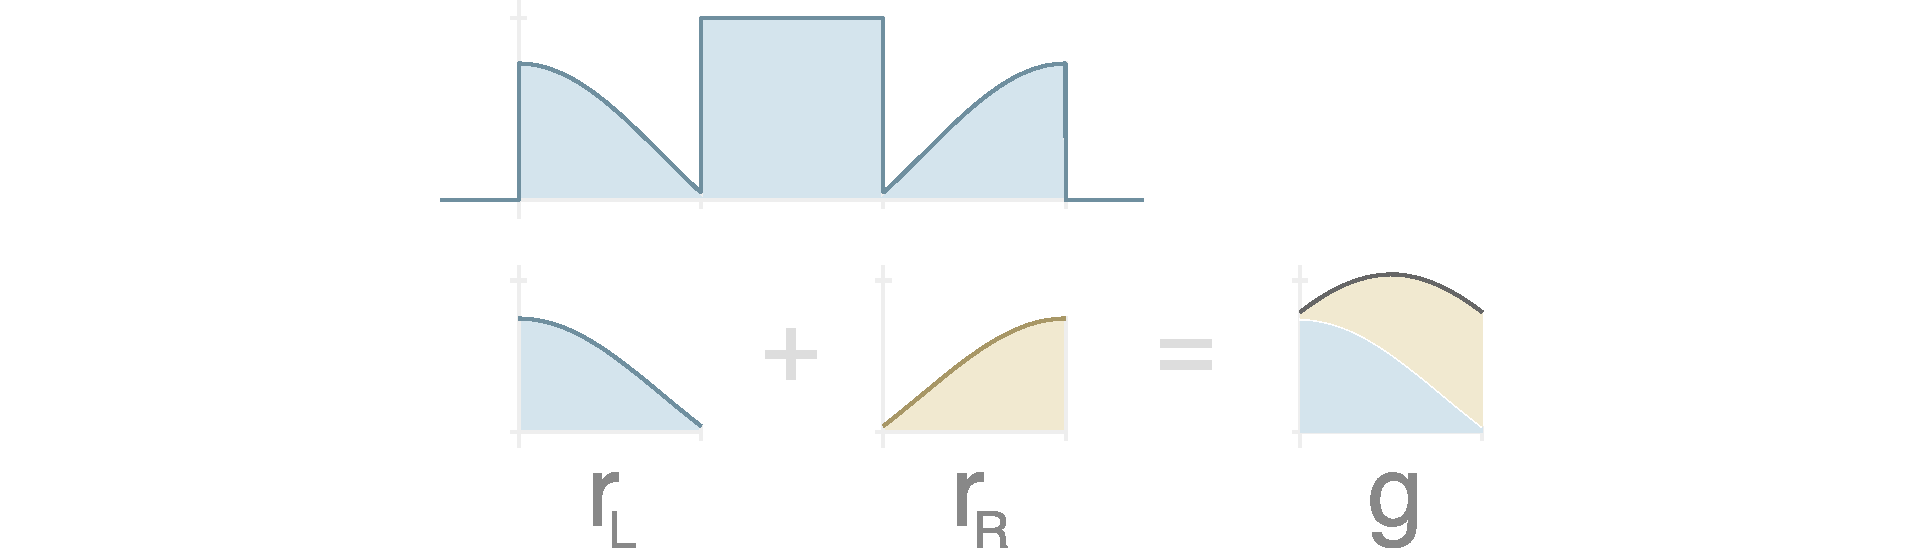
\includegraphics{images/pdfs/nonpl_setup.pdf}
\caption{\label{fig:nonpl_setup}An example showing how \(r_L\), \(r_R\),
and \(g\) are extracted from a function
\(f\).}\label{fig:nonplux5fsetup}
\end{figure}

TODO Clean up the font used in this image (looks bad in the pdf right
now).

I'll show that the shape of \(g\) must dominate the landscape of \(f\)
in order for it to be exactly self-replicating.

Now suppose that \(f\) is exactly self-replicating. I'll use definition
(\ref{eq:exact_defn}) to provide functions \(f_L\), \(f_R\), and \(f_S\)
in terms of \(f\), \(s\), \(t_1\), and \(t_2\). Notice that

\[\big(f_S \restrict [2,3]\big) = \big(f_L + f_R \restrict [2, 3]\big) =
r_L + r_R = g.\]

Since \(f_L(x) = f_S(t_1(x))\), and \(t_1\) maps \([2,3]\) to
\([1\tfrac{1}{3}, 1\tfrac{2}{3}]\), this means
\((\,f_L \restrict [1\tfrac{1}{3}, 1\tfrac{2}{3}]) = g\).

\newcommand{\zerotwo}{\raise1.5pt\hbox{$\genfrac{}{}{0pt}{}
{\lower1.8pt\hbox{$\smash{\scriptstyle 0}$}}
{\raise0pt\hbox{$\smash{\scriptstyle 2}$}}$}}

%\newcommand{\zerotwo}{{\lower1em\hbox{$\smash{0}$}\atop\hbox{$\smash{2}$}}}

At this point it will be useful to begin using base-3 notation for the
intervals at hand. If \(s\) is a finite string with digits from the set
\(\{0, 1, 2\}\), then let \(0.s\overline{*}_3\) denote the closure of
the set of points whose base-3 expansion begins with \(0.s\). For
example, \(0.11\overline{*}_3\) denotes the interval
\([0.11_3, 0.12_3]\) while \(0.012\overline{*}_3\) denotes the interval
\([0.12_3, 0.20_3]\). I'll also use \(\zerotwo\) to denote a digit that
may be either a 0 or a 2; for example, \(0.1\zerotwo 1\overline{*}_3\)
denotes the union of intervals \([0.101_3, 0.102_3]\) and
\([0.121_3, 0.122_3]\).

Now, instead of writing
\((\,f_L \restrict [1\tfrac{1}{3}, 1\tfrac{2}{3}]) = g\), I can write
\((\,f_L \restrict 1 + 0.1\overline{*}_3) = g\). This means that
\((\,f_R \restrict 3 + 0.1\overline{*}_3) = g\), so that
\((\,f_S \restrict \{1,3\} + 0.1\overline{*}_3) = g\). As above, use the
map \(t_1\) to conclude that
\((\,f_L \restrict 0.\zerotwo 1\overline{*}_3) = g\).

TODO work up to this image

\begin{figure}[htbp]
\centering
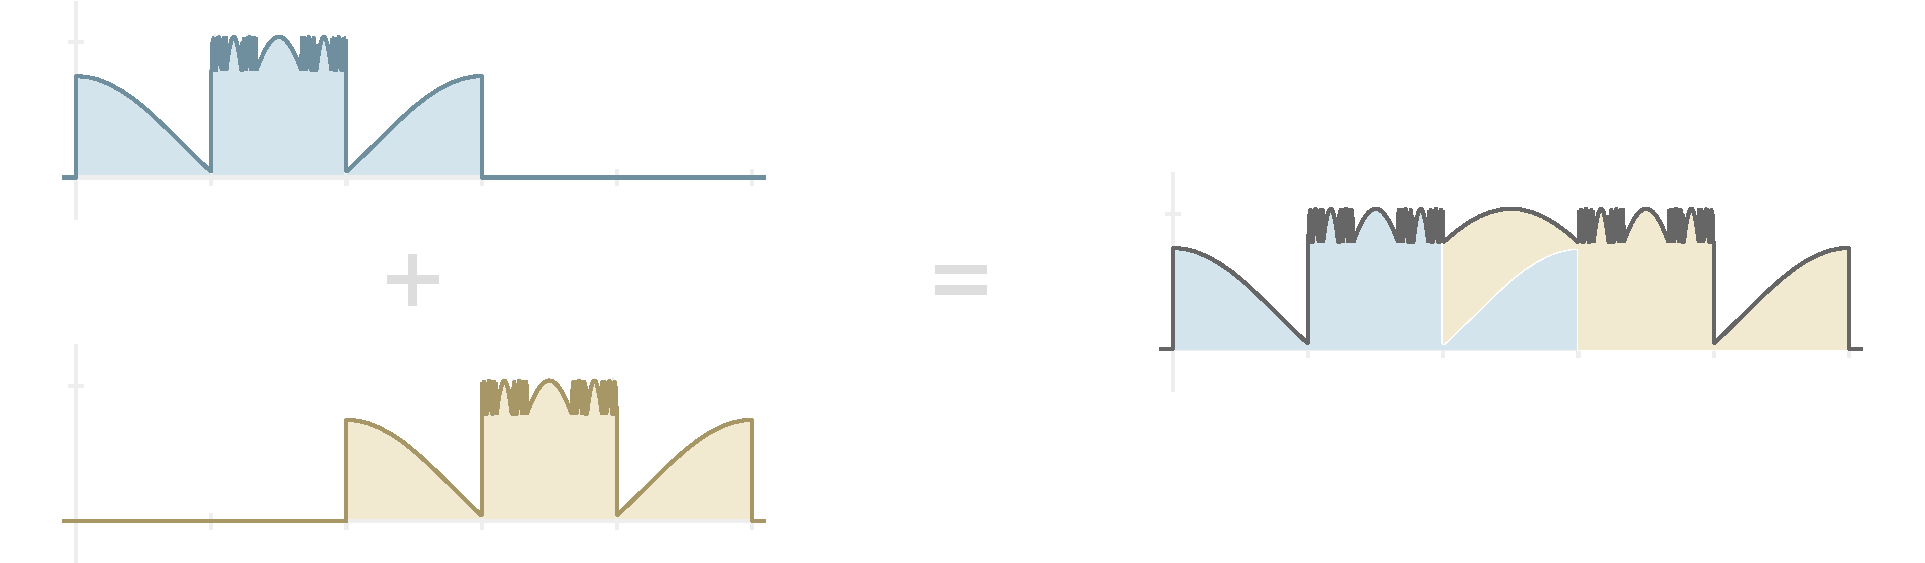
\includegraphics{images/pdfs/nonplateau.pdf}
\caption{\label{fig:nonplateau}An exactly self-replicating function
\(f\) completely determined by \(r_L(x) = \cos(2x)/2 + 1/4\),
\(r_R(x) = r_L(1 - x)\), and the value \(f(x) = r_L(0) + r_R(0)\) for
all \(x\) not determined by \(r_L\) and \(r_R\).}\label{fig:nonplateau}
\end{figure}

TODO Clarify the values of \(s\), \(t_1\), and \(t_2\) in that caption.

\begin{center}\rule{0.5\linewidth}{\linethickness}\end{center}

\subsubsection{\texorpdfstring{All possible positive curves for the
example \(s,t_1,t_2\)
parameters}{All possible positive curves for the example s,t\_1,t\_2 parameters}}\label{all-possible-positive-curves-for-the-example-stux5f1tux5f2-parameters}

Consider a general function \(f(x)\) such that \(f(x)=0\) except when
\(x \in [0, 5]\). For convenience, I'll introduce the notation
\(\alpha_{[0,1]}\) to denote the function

\[\alpha_{[0,1]}(x) = \alpha(x) \cdot \big[ x\in [0,1] \big],\]

for any function \(\alpha(x)\). Using this notation, it will be useful
to isolate the left and right ramps \(r_L(x) = f_{[0,1]}(x)\) and
\(r_R(x) = \big(f(x + 4)\big)_{[0,1]}\).

\begin{center}\rule{0.5\linewidth}{\linethickness}\end{center}

TODO finish from here; don't forget that \(s\) can't be the identity
function

\subsubsection{Begin other stuff to
rewrite}\label{begin-other-stuff-to-rewrite}

I'll describe a sequence of functions which may help us find a
self-replicating function by starting with an arbitrary function. The
sequence depends on an initial function \(f(x)\), a shift function
\(s(x)\) that captures the relationship between the left and right
addends, and transformation functions \(t_1(x)\) and \(t_2(x)\) that
formalize the similarity between the addends and their sum.

Given these functions, we can define

\[\begin{array}{rcl}
  f_L(x) & = & f(x), \\
  f_R(x) & = & f(s(x)), \text{and} \\
  f_S(x) & = & f_L(x) + f_R(x), \\
\end{array}\]

with the expectation that

\[f_L(x) = t_2(f_S(t_1(x))).\]

This setup supports the possibility that \(f_L\) and \(f_R\) are
possibly-reflected shifts of each other, and requires \(f_S\) can be
transformed to recover exactly \(f_L\). This is one possible way to
formalize the definition of a self-replicating function.

It can also be used to set up a sequence of functions via the following
definitions:

\[\begin{array}{rcl}
  f^{(1)}_L & = & f(x), \\
  f^{(i)}_R & = & f^{(i)}_L \\
  f^{(i+1)}_S = f^{(i)}_L + f^{(i)}_R \\
\end{array}\]

TODO finish the above

\section{The normal curve}\label{the-normal-curve}

The normal curve is described by \(y = e^{-x^2/2}\).

\begin{figure}[htbp]
\centering
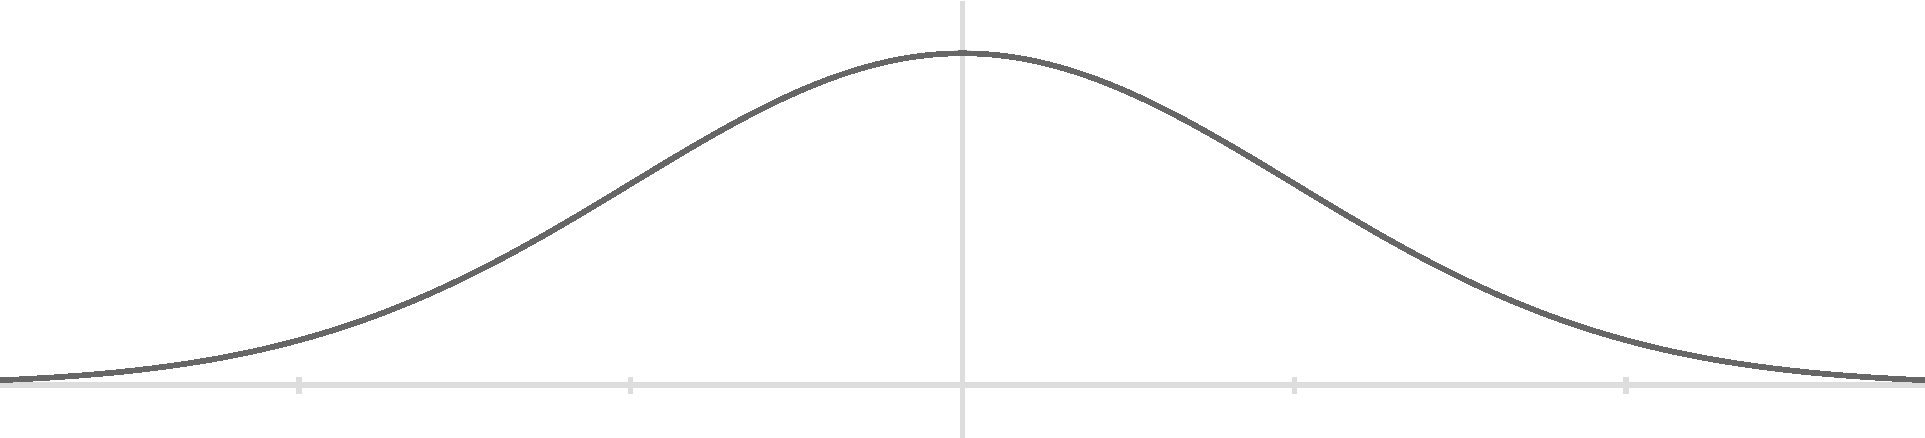
\includegraphics{images/pdfs/normal3.pdf}
\caption{The normal curve: \(y=e^{-x^2/2}\).}
\end{figure}

\section{\texorpdfstring{Leaf-point distributions of
\emph{L}-systems}{Leaf-point distributions of L-systems}}\label{leaf-point-distributions-of-l-systems}

\section{Fractal functions}\label{fractal-functions}

This section is for functions similar to the Cantor diagonal. It may
turn out that I can't find any functions that fit here, or that the
\emph{L}-systems distributions includes this case, or even that I can
prove that no functions could exist here (as far as I know).

TODO Add a note somewhere that the initial setup requires that the sum
itself is always the translation of an even function.

\section{Temporary example content}\label{temporary-example-content}

\textbf{Lemma 1}~ \emph{Content of lemma 1, including some \(\pi+3\)
mathy bits.}

\subsection{Subheader}\label{subheader}

Content

See my notes on Raney's lemmas for more examples.

Here is a reference (Knuth, Patashnik, and Graham 1997).

\section{Questions}\label{questions}

\begin{itemize}
\tightlist
\item
  The ellipse around my first \emph{L}-system appears to fit
  surprisingly well. Is there a nice way to discover when an ellipse and
  an \emph{L}-system may fit like this? Is there, perhaps, a series of
  shapes which converge on the system or its leaf points, analogous to
  \href{http://mathworld.wolfram.com/MandelbrotSetLemniscate.html}{Mandelbrot
  set lemniscates}?
\item
  The histogram around my first \emph{L}-system appears simple in shape.
  Can its shape be described precisely?
\item
  The sigmoid \(\sigma(x)=1/(1+e^{-x})\) provides a
  near-self-replicating split of \(e^{-x^2}\). Is there a function
  \(f(x)\) such that \(\sigma(x)\) provides an \emph{exact}
  self-replicating split? More than one? In general, given any sigmoid
  \(s(x)\), what is the set of functions which it splits exactly in this
  way? For this question, we can have some precise requirement for a
  sigmoid, such as being an appropriately scaled and translated odd
  function.
\item
  Are there variants of self-replicating functions that work for other
  sets of operations such as using more than two copies of the function
  in a sum, or by using multiplication or some other operation instead
  of addition?
\end{itemize}

\section*{References}\label{references}
\addcontentsline{toc}{section}{References}

\hypertarget{refs}{}
\hypertarget{ref-taocp1}{}
Knuth, Donald E. 1998. \emph{Fundamental Algorithms}. Third Ed. Vol. 1.
The Art of Computer Programming. Addison-Wesley.

\hypertarget{ref-concrete}{}
Knuth, Donald E., Oren Patashnik, and Ronald L. Graham. 1997.
\emph{Concrete Mathematics: A Foundation for Computer Science}.
Addison-Wesley.

\end{document}
